\chapter{Fundamentação Teórica}

% Esse capitulo visa introduzir alguns dos conceitos e componentes vinculados aos tópicos de aprendizado de máquina e aprendizado profundo, com enfoque nas aplicações de detecção e reconhecimento de texto.

\section{Aprendizado de Máquina e Aprendizado Profundo}
O aprendizado de máquina é uma área dentro do amplo espaço de estudo que é tocado pela campo de Inteligencia Artificial. O aprendizado de máquina, envolve o estudo e aplicação de algoritmos que são especialistas em reconhecer padrões em base de dados, muitas vezes não triviais para uma analise humana [\citeonline{MLDLVision}], e são capazes de, a partir da recorrente exposição a esses dados e aos padrões identificados, responder perguntas e predizer informações sobre novos dados nunca antes vistos. O aprendizado profundo uma vertente dentro da área de aprendizado de máquina e decorre a partir das redes neurais artificiais profundas, ou seja, com mais camadas ocultas entre a entrada e a saída da rede.

Uma das grandes diferenças entre aprendizado profundo e aprendizado de máquina é como a representação e extração de características é automatizada em métodos de aprendizado profundo. A maior profundidade das redes permite que características de diferentes níveis de abstração sejam montadas pelos diferentes níveis da rede [\citeonline{DeepLearningATA}], o que contrasta bastante com a geral necessidade de etapas pré-processamento sobre os dados de entrada de algoritmos de aprendizado de máquina para a montagem de características [\citeonline{MLDLVision, ReviewDL}]. A Figura \ref{fig:dl_vs_ml} ilustra em alto nível essa diferença entre aprendizado de máquina e aprendizado profundo.

\begin{figure}
    \centering
    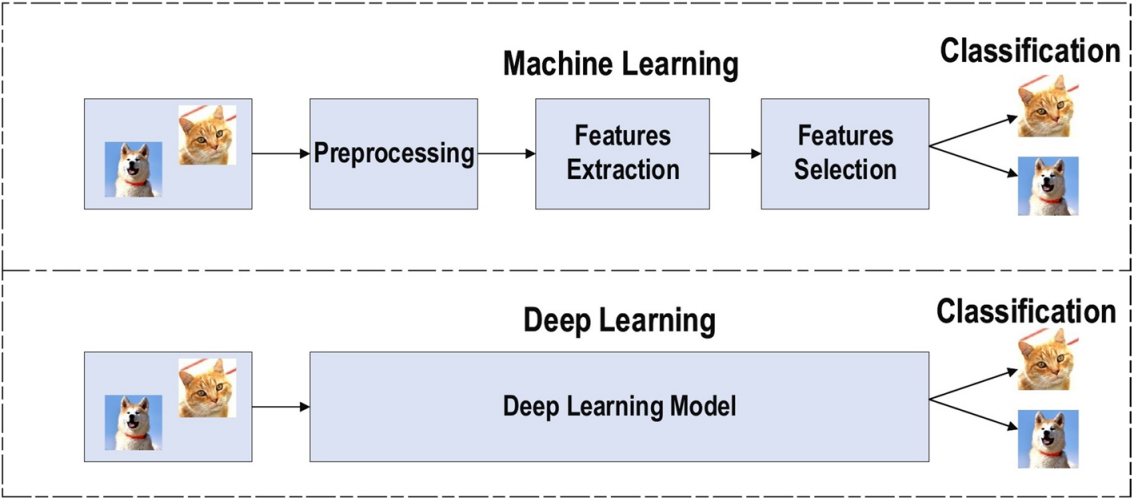
\includegraphics[width=0.8\textwidth]{figs/theory-ml-vs-dl.png}
    \caption{Diferenças em alto nível entre aprendizado profundo e aprendizado de máquina referente às etapas de processamento. Fonte [\citeonline{ReviewDL}]}
    \label{fig:dl_vs_ml}
\end{figure}

Técnicas e algoritmos, tanto de aprendizado de máquina quanto de aprendizado profundo, podem ser basicamente classificados em diferentes grupos [\citeonline{ReviewDL}]:
\begin{itemize}
    \item Algoritmos de aprendizado supervisionado: Baseiam-se na exposição de um grande volumes de exemplos devidamente anotados, isso é, cada exemplo que será consumido pelo modelo em treinamento deve conter também o resultado que é esperado na saída do algoritmo, para que seja possível a comparação entre o resultado do modelo contra o valor de gabarito. A partir dessa comparação tem-se o eventual erro de predição, que é iterativamente utilizado pelo algoritmo para refinar suas respostas em geral com no processo chamado de \textit{back-propagation}.
    \item Algoritmos de aprendizado semi-supervisionado: Assim como o nome sugere, é uma abordagem válida quando não existe grande volume de dados com as anotações necessárias. Ainda assim, a depender da aplicação, a existência de um volume menor de dados anotados pode ser melhor do que nenhum dado anotado, portanto ainda possuem grande valor no treinamento.
    \item Algoritmos de aprendizado não supervisionado: É aplicável quando não existe bases de dados em volume com exemplos anotados. Dessa forma, o próprio algoritmo vai tentar derivar relacionamentos entre exemplos a fim de encontrar características intrínsecas aos dados de entrada.
\end{itemize}

Duas estruturas bastante populares de aprendizado profundo, as redes neurais convolucionais e as redes neurais recorrentes, serão abordadas nas próximas seções. Ambas são base dos métodos de detecção e reconhecimento de texto utilizados ao longo do trabalho de graduação.

%%%%%%%%%%%%%%%%%%%%%%%%%%%%%%%%%%%%%%%%%%%%%%%%%%%%%%%%%%%%%%%%%%%%%%%%%%%%%%%%

\subsection{Redes Neurais Convolucionais}
As redes neurais convolucionais, abreviadas por CNN pelo nome em inglês \textit{Convolutional Neural Network}, é um modelo de rede neural que tem inspiração no córtex visual animal, uma estrutura cerebral que processa os estímulos visuais originados a partir dos olhos. Apesar da inspiração e o foco inicial em problemas de visão computacional, atualmente é um conceito já aplicado em outros segmentos de pesquisa, como processamento de sinais, processamento de voz e linguagem, para citar algumas dessas aplicações. [\citeonline{ReviewDL, 1DCNN}]

\begin{figure}
    \centering
    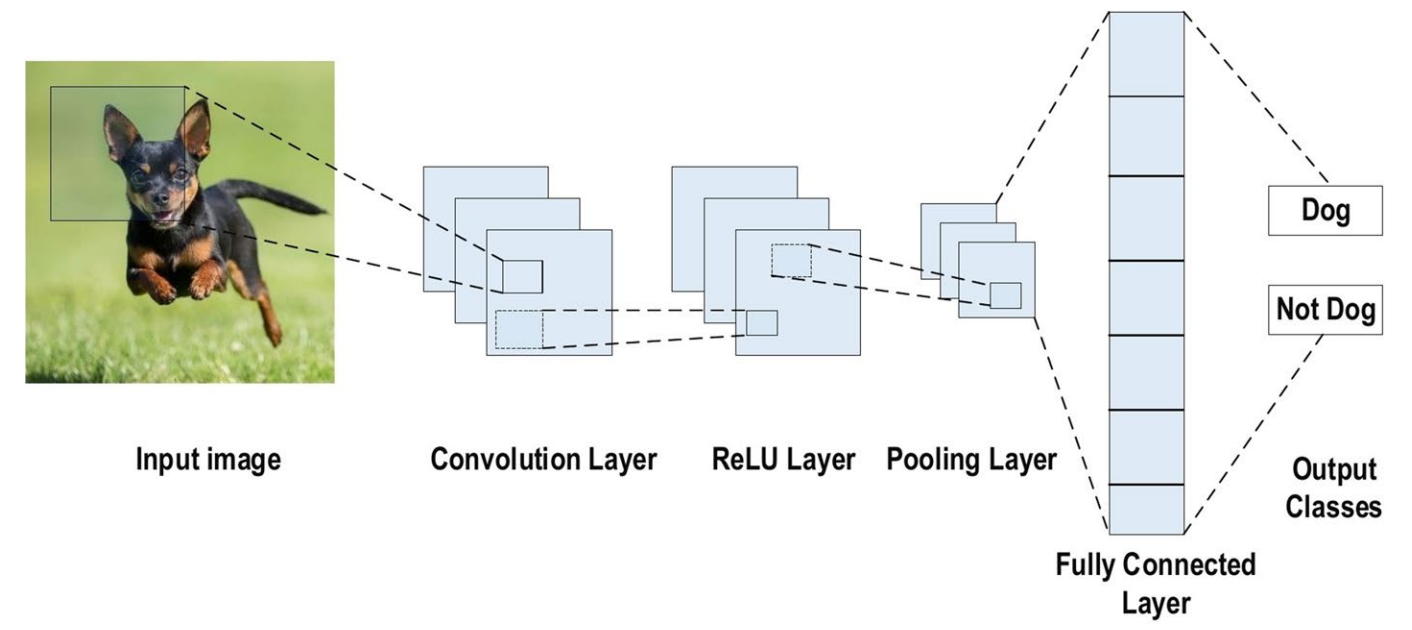
\includegraphics[width=0.8\textwidth]{figs/theory-cnn-example.png}
    \caption{Exemplo de rede convolucional, ilustrando as camadas ocultas da rede neural. Fonte [\citeonline{ReviewDL}]}
    \label{fig:theory-cnn-example}
\end{figure}

As arquiteturas de redes convolucionais mais comuns são, em geral, composições de diferentes de três tipos de camadas, observáveis a partir da Figura \ref{fig:theory-cnn-example}, cada uma com um propósito específico:
\begin{enumerate}
    \item \textbf{Camada de Convolução}:
            A camada de convolução tem como papel processar a imagem de entrada e extrair mapas de características baseado na aplicação de diferentes filtros bi-dimensionais (ou \textit{kernels}) sobre a imagem em uma operação de convolução, de forma análoga ao uso de filtros morfológicos, no âmbito de processamento de imagem. Para cada filtro aplicado nas camadas de convolução, uma nova representação dos dados de entrada é gerada, que é comumente chamado de mapa de características (mapa de característica). As camadas mais rasas em geral conseguem entender características de mais alto nível, menos abstratas, por estarem mais próximas da entrada de dados. Camadas mais profundas extraem características mais abstratas, já que são ativadas por mapas de características provenientes das camadas mais rasas [\citeonline{IntoMLNNDL}].
        
            A introdução de não-linearidade nas redes convolucionais decorre da aplicação de funções de ativação, normalmente ao final da operação de convolução. A função de ativação mais comum é a ReLU (\textit{Rectified Linear Unit}, em inglês), sendo um dos motivos a sua eficiência computacional quando comparada a outras funções de ativação [\citeonline{ActvFunc}], como $sigmod$ e $tanh$. A Equação \ref{eq:relu} apresenta a definição matemática da função de ativação ReLU.
            
            \begin{equation}
                f(u) = max(0,u)
                \label{eq:relu}
            \end{equation}
            
            Ainda sobre a camada de convolução, existem quatro hiper-parâmetros que uma breve introdução se faz necessária:
            \begin{itemize}
                \item \textbf{Stride}: É o passo da aplicação do filtro sobre a imagem. \textit{Stride} igual a um significa que a convolução vai percorrer a imagem de pixel em pixel
                \item \textbf{Receptive-Field}: É o tamanho dos filtros aplicados à imagem. \textit{Receptive-Field} igual a dois significa que os filtros têm dimensões 2x2 pixels.
                \item \textbf{Depth}: É a profundidade de cada mapa de características e está diretamente relacionado ao número de filtros que são aplicados à imagem.
                \item \textbf{Zero-Padding}: É a espessura da borda de zeros que deve ser aplicada na imagem pré-convolução. Durante a concepção de um modelo de CNN, é importante levar em consideração as dimensões da imagem de entrada e dos mapas de características de cada camada de convolução. É importante que os filtros consigam percorrer a imagem sem extrapolar nenhum índice durante as iterações. Aplicar o valor correto de \textit{Zero-Padding} e \textit{Stride} faz com que o tamanho dos mapas de características sejam bastante previsíveis, o que facilita a modelagem.
            \end{itemize}
            
    \item \textbf{Camada de Pooling}:
            A camada de \textit{pooling} é responsável por fazer o \textit{down-sampling} dos mapas de características, ou seja, reduz a dimensão desses mapas, o que em geral melhora o desempenho de convergência modelo, potencializa a generalização do que está sendo aprendido controlando o problema de \textit{over-fitting}, diminuindo o número de parâmetros e ativações do modelo.
            
            A configuração mais comum de uma camada de \textit{pooling} é o de filtros com \textit{Receptive-Field} igual a dois aplicados com \textit{Stride} igual a dois. Isso faz com que o mapa de características tenha sua altura e largura diminuídas pela metade, dessa forma reduzindo em 75\% sua complexidade em quantidade de parâmetros da rede [\citeonline{StanfordCNN}].
            
            Para saber os novos valores de ativação do mapa reduzido, a operação mais comum executada durante o processo de convolução a operação $max$ ou $average$, com o intuito de conservar as ativações mais predominantes de cada mapa de características.
            
    \item \textbf{Camada de Totalmente Conectada}:
            A camada \textit{fully-connected} é bastante comum de ser aplicada no final do pipeline de processamento de uma arquitetura de CNN pela sua capacidade de decisão. Essa camada é mais parecida com a estrutura comum de redes neurais artificiais, onde existe uma ou mais camadas de neurônios que recebem parcelas de ativação de todos os nós da camada anterior.
            
            Em problemas de classificação, essa camada é responsável por abstrair as características extraídas por camadas ocultas anteriores em valores de probabilidade, a fim de formalizar o resultado da predição [\citeonline{DeepLearningATA}]. A operação mais comum na saída da camada totalmente conectada é o $softmax$, exposta pela Equação \ref{eq:softmax}.
            
            \begin{equation}
                \label{eq:softmax}
                softmax(y_j) = \frac{exp(y_j)}{\sum exp(y_j)}
            \end{equation}
            
            Apesar de ser um componente bastante comum em arquiteturas de redes convolucionais, as camadas totalmente conectadas nem sempre estão presentes. Dependendo do propósito da rede, pode-se omitir a camada de classificação totalmente conectada e substituir por novas camadas de convolução com filtros de dimensão 1x1 pixels para fazer o mesmo trabalho de classificação ou ainda usar novas camadas de de-convolução e \textit{up-sampling} para a saída da rede ser uma imagem segmentada semanticamente [\citeonline{FCN}]. Redes convolucionais que não contam com as últimas camadas densas e utilizam camadas convolucionais no seu lugar são normalmente chamadas de FCN, \textit{Fully-Convolutional-Networks}.
\end{enumerate}

Quando aplicado a entradas visuais em forma de imagens, o tamanho final do modelo treinado e o número total de parâmetros de uma rede CNN é menor se comparada com uma rede neural convencional. Em [\citeonline{IntroCNN}] é exemplificado uma rede neural convencional, por em geral serem densas, ou seja, os neurônios das camadas da rede são todos interligados, o número de parâmetros treinados da rede cresce muito rápido com as dimensões da imagem de entrada. Em contrapartida, nas redes convolucionais, cada nó da rede é ativado por uma secção da imagem de entrada, descrito pelo hiper-parâmetro \textit{Receptive-Field}, dessa forma, na operação de convolução, cada neurônio da rede tem a responsabilidade de identificar características de secções distintas da imagem de entrada.

A partir do uso dos componentes mais comum e básicos de uma rede convolucional em diferentes composições, é possível configurar arquiteturas mais complexas. Alguns trabalhos ao longo dos últimos anos exploraram bastante novas arquiteturas de redes convolucionais, como por exemplo VGG [\citeonline{VGG}], ResNet [\citeonline{ResNet}] e GoogLeNet [\citeonline{GooLeNet}]. Uma base de imagens bastante utilizada por alguns desses trabalhos é o ImageNet [\citeonline{ImageNet}], que contém vasto número de exemplos que são base de uma competição de detecção e classificação de objetos, ILSVRC (\textit{ImageNet Large Scale Visual Recognition Challenge}) [\citeonline{ILSVRC}]. Unindo a robustez e capacidade de representação de características das CNN com a alta exposição a diversos exemplos através do ImageNet, as redes melhores colocadas no ILSVRC ao longo dos anos se tornaram referência em extração de características e, em diversos casos [\citeonline{CRAFT, CRNN}], são utilizadas em soluções de contexto mais específicos justamente através de técnicas como o \textit{transfer-learning} [\citeonline{TransfLearn}].

%%%%%%%%%%%%%%%%%%%%%%%%%%%%%%%%%%%%%%%%%%%%%%%%%%%%%%%%%%%%%%%%%%%%%%%%%%%%%%%%%%%%%%%%%%%%%%%%%%%%%%%%%%%%%%%%%%%%%%%%

\subsection{Redes Neurais Recorrentes}
As redes neurais recorrentes, abreviadas por RNN (\textit{Recurrent Neural Networks}, em inglês) são bastante populares no contexto de processamento de linguagem natural devido ao seu caráter de conseguir processar dados sequenciais [\citeonline{ReviewDL}]. A principal característica das redes RNN é que a predição no instante de tempo $T$ é estimulada pelo dado de entrada e pelo estado interno da rede no instante de tempo passado, $T - 1$. De maneira simplista, essa característica se assemelha ao conceito de memória, onde a rede sempre considera tudo o que já foi processado em momentos anteriores para compor resultado do momento corrente, carregando o contexto ao longo do tempo.

\begin{figure}
    \centering
    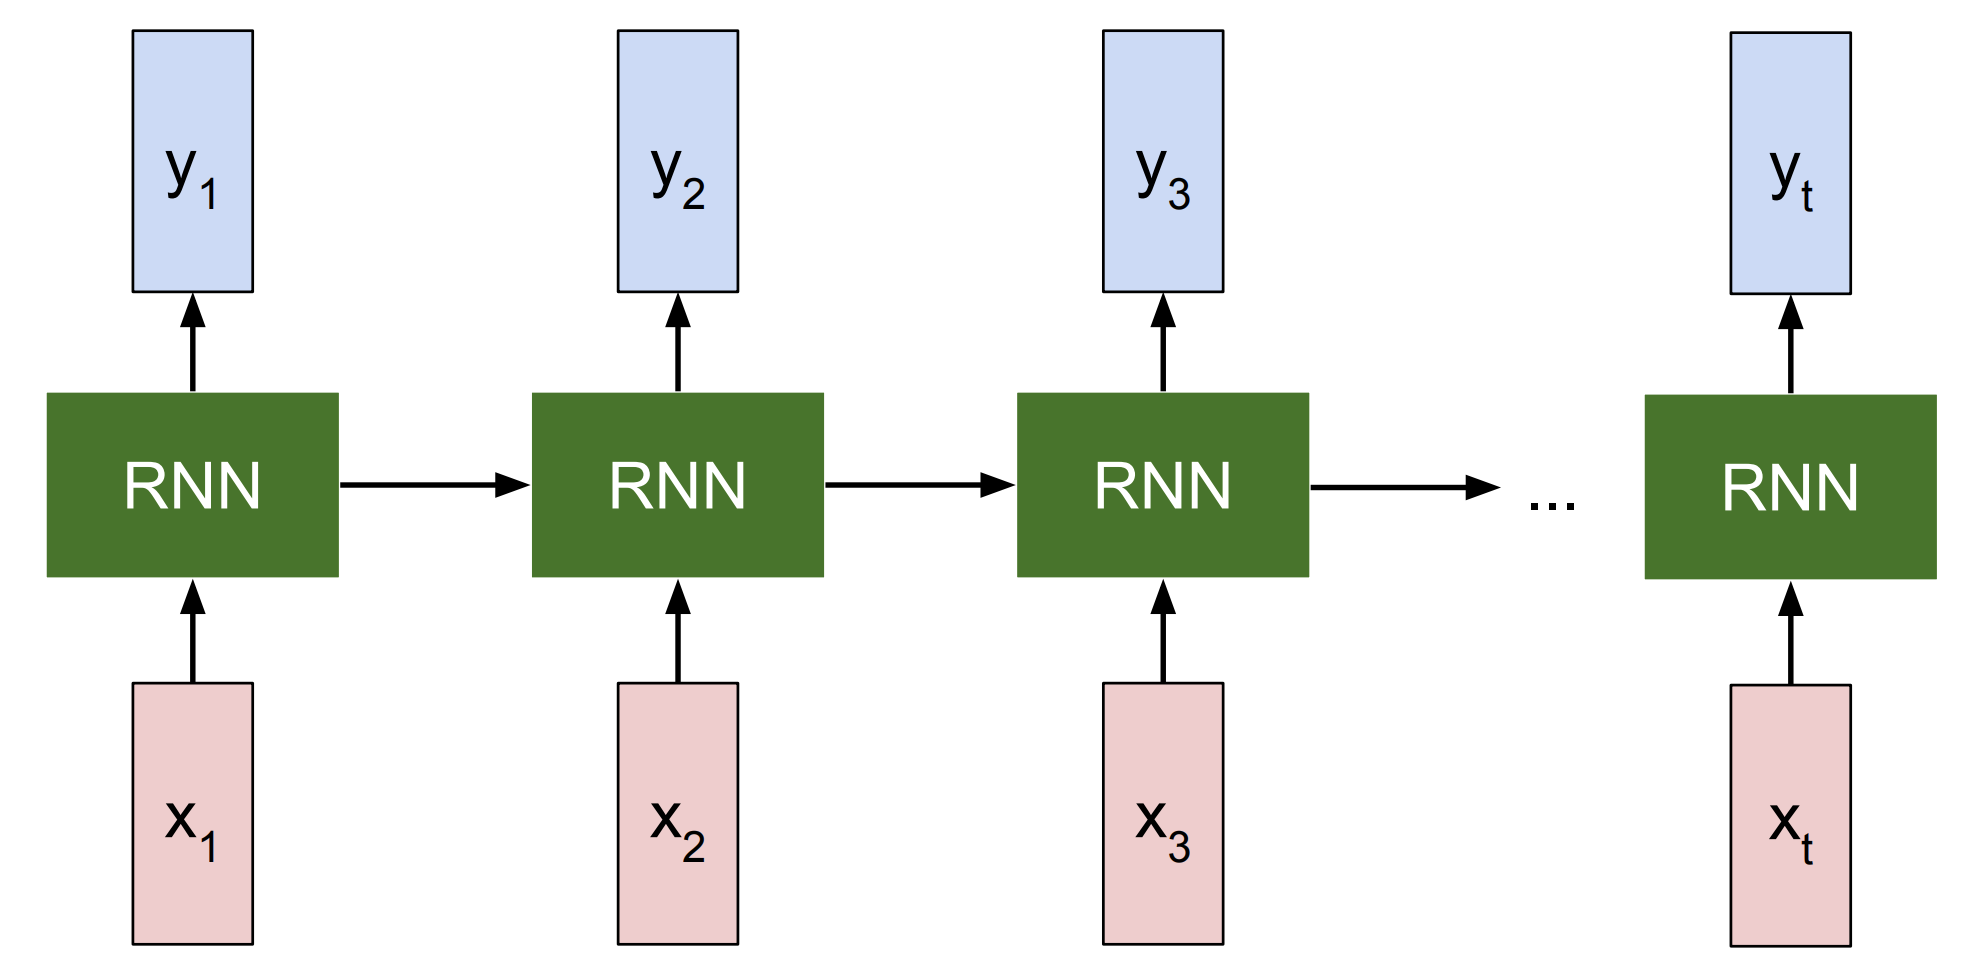
\includegraphics[width=0.8\textwidth]{figs/theory-example-rnn.png}
    \caption{Ilustração de um exemplo de rede neural recorrente. Fonte [\citeonline{StanfordRNN}]}
    \label{fig:theory-rnn-example}
\end{figure}

A versão dita canônica das redes neurais recorrentes tem sua estrutura ilustrada pela Figura \ref{fig:theory-rnn-example}, onde é possível observar que a representação aberta da rede se assemelha a uma cadeia de "neurônios" conectados. O fator de não-linearidade deriva do uso de funções como $tanh$, $sigmoid$ e ReLu durante a computação do estado interno da rede em cada instante de tempo. As redes recorrentes também podem ser compostas em configurações diferentes, onde dois exemplos são redes recorrentes profundas, duas ou mais RNNs empilhadas [\citeonline{DRNN}], e redes recorrentes bi-direcionais [\citeonline{BRNN}], profundas ou não, que tenta lidar com problemas onde o contexto a priori e a posteriori são importantes.

Apesar das redes neurais recorrentes, na sua forma original, terem a capacidade de lidar com entradas e saídas sequenciais de tamanhos arbitrários, empiricamente demonstrou problemas ao lidar com sequências muito longas, principalmente uma grande sensibilidade aos problemas de explosão e desaparecimento de gradiente em métodos de treinamento baseados em propagação do erro de predição [\citeonline{VanishGrad}]. Para lidar com esse problema, novas variantes de redes recorrentes foram idealizadas, sendo a que mais se popularizou foi a LSTM, que é a abreviação para \textit{Long Short-Term Memory} [\citeonline{LSTM}].

A principal mudança entre a rede RNN convencional para a rede LSTM foi a introdução de uma nova estrutura capaz de aprender a preservar contexto histórico na rede e podem ser interpretados como células de memória. A partir de novos meios treináveis de adicionar, preservar e limpar informações dessa célula, a rede se tornou muito mais capaz e eficiente na gestão dos parâmetros responsáveis por segurar o contexto histórico da rede, mitigando os problemas de \textit{Vanishing} e \textit{Exploding Gradients}. 

%%%%%%%%%%%%%%%%%%%%%%%%%%%%%%%%%%%%%%%%%%%%%%%%%%%%%%%%%%%%%%%%%%%%%%%%%%%%%%%%%%%%%%%%%%%%%%%%%%%%%%%%%%%%%%%%%%%%%%%%

\section{Evolução do \textit{Scene Text Recognition}}
\textit{Optical Character Recognition}, abreviado por OCR, e mais especificamente Scene Text Recognition, abreviado por STR, podem ser atacados como um sub-conjunto de problemas de identificação de objetos [\citeonline{DetcRecogWild, StrDlEra}] e esse fato trouxe diversas adaptações de métodos mais clássicos de detecção de objetos para o contexto de detecção de texto. A forma mais convencional de OCR, a detecção de texto manuscrito ou impresso, apesar de ser desafiador (em especial o caso de manuscritos), é tido como muito bem resolvido, com soluções de sucesso aplicadas em larga escala [\citeonline{DetcRecogWild, WhatIsWrongSTR}], em grande parte por apresentarem um contexto mais simples onde o texto está inserido, com planos de fundo mais consistentes, com menos ruídos, e padrões de mais fácil detecção quando comparado ao casos de STR.

Apesar da introdução sobre as redes convolucionais na seção anterior e a breve menção que as redes neurais convolucionais são amplamente utilizadas no espoco de problemas de detecção e reconhecimento de texto atualmente, vale mencionar que nem sempre foi assim. Trabalhos que estudaram e resolveram a detecção e reconhecimento de texto já eram feitos mesmo antes da ampla popularidade do aprendizado profundo e aliavam métodos de extração de características, mais artesanais e específicos para o contexto de aplicação, com modelos e algoritmos de aprendizado de máquina ditos clássicos para a fazer a classificação/predição.

Em [\citeonline{DetcRecogWild, StrDlEra}] é exposto que o processo de interpretação de texto contidos em imagens é composto por duas grandes etapas: A localização e/ou detecção do texto e o reconhecimento do texto. A etapa de detecção e/ou localização visa justamente responder se, dada uma imagem, existe texto nela e, caso positivo, adequadamente localizá-lo. Já o reconhecimento tem a responsabilidade de interpretar o texto contido na imagem, a fim de conseguir transformar regiões de texto em sequências de caracteres que possam ser utilizados por computadores.

A partir dessa interpretação, nessa seção será feita uma breve revisão bibliográfica abordando a evolução das soluções de detecção e reconhecimento até a popularização dos métodos de aprendizado profundo. Serão abordados em maior detalhes dois trabalhos, um sobre detecção e outro sobre reconhecimento, pois farão parte do desenvolvimento prático deste trabalho de graduação.

%%%%%%%%%%%%%%%%%%%%%%%%%%%%%%%%%%%%%%%%%%%%%%%%%%%%%%%%%%%%%%%%%%%%%%%%%%%%%%%%%%%%%%%%%%%%%%%%%%%%%%%%%%%%%%%%%%%%%%%%

\subsection{Detecção de Texto}
Em momentos anteriores ao grande crescimento de popularidade do aprendizado profundo, as soluções de detecção de texto em cenas precisavam de profunda análise e manuseio das imagens para conseguir identificar padrões em torno do problema a ser resolvido para que então fosse possível, manualmente, construir e descrever uma série de características que seriam a base para identificar o texto na imagem. Todo esse processo é bastante artesanal, consumindo muito tempo humano, e as características produzidas em geral são bastante especializadas no contexto de atuação, como citado por [\citeonline{DeepLearningATA}], ou seja, o reuso de uma característica montada no contexto de detecção de texto em outros problemas, como por exemplo o processamento de linguagem natural, seria difícil.

Para o problema de detecção de texto, ainda no período anterior ao uso do aprendizado profundo, [\citeonline{DetcRecogWild, StrDlEra}] constatam que é possível, de maneira geral, agrupar as soluções baseadas em aprendizado de máquina clássico em duas categorias:
\begin{itemize}
    \item Soluções baseadas no conceito CCA (\textit{Connected Components Analysis}, em inglês), que se baseiam em agregar regiões da imagem que compartilham características, como por exemplo, cor, textura e extremidades [\citeonline{SurveyImagery}]. Dois trabalhos com bastante evidencia nesse segmento são os que originaram os métodos \textit{Stoke Width Transform} (SWT) [\citeonline{SWT}] e \textit{Maximum Stable Extremal Regions} (MSER) [\citeonline{MSER}].
    \item Soluções baseadas no conceito de SW, abreviação do nome em inglês \textit{Sliding Windows}, que se baseiam em percorrer a imagem com janelas, de diferentes tamanhos, e, de forma simplista, aplicando testes para a existência ou não de texto na área da janela observada em conjunto a um método classificador, treinados para detectar texto baseado em características construídas para tal.
\end{itemize}

A introdução de técnicas de aprendizado profundo na solução da detecção de texto expandiu o leque de possibilidades em torno de como lidar com o problema, o que movimentou bastante pesquisas sobre o tema, o que pode ser constatado com o número de novos trabalhos abordando o problema nas últimas duas décadas. Inicialmente, os primeiros trabalhos que aplicavam redes neurais as utilizavam como meio de extração de características, substituindo grande parte do processo de engenharia de características específicas, para posteriormente aplicar os métodos de processamento de imagens e visão computacional já conhecidos.

Posteriormente, alguns conceitos e técnicas mais gerais de detecção de objetos foram trazidos para o contexto de reconhecimento de texto, o que criou, de acordo com [\citeonline{DetcRecogWild}], três linhas de solução para o problema de detecção de texto, ilustradas na Figura \ref{fig:theory-detection-categories}:

\begin{figure}
    \centering
    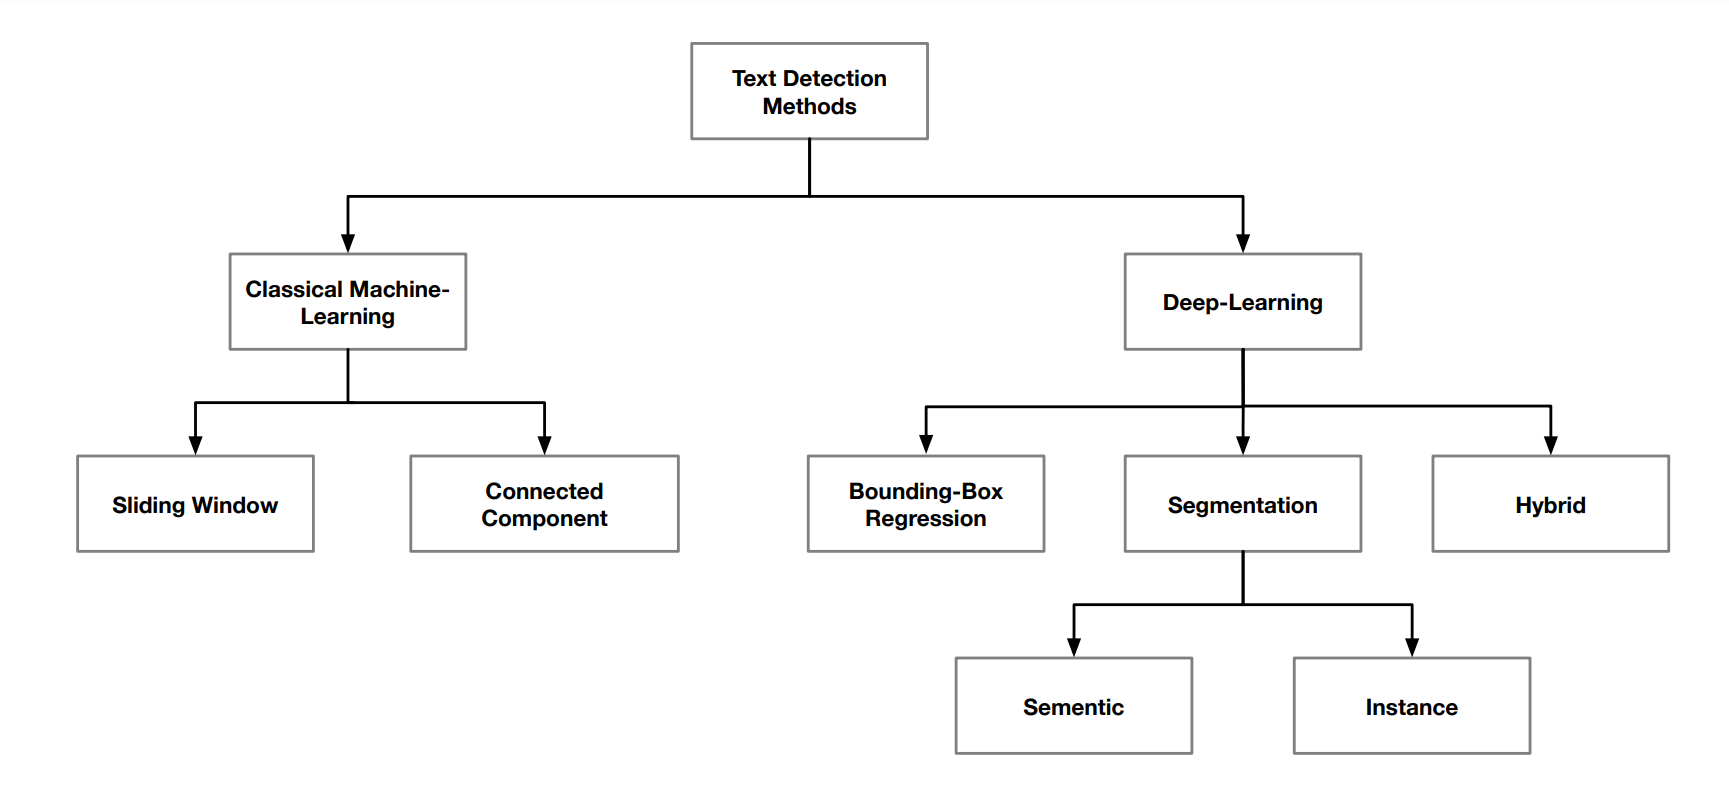
\includegraphics[width=\textwidth]{figs/theory-detection-categories.png}
    \caption{Categorias de abordagens na solução de detecção de texto. Fonte [\citeonline{DetcRecogWild}]}
    \label{fig:theory-detection-categories}
\end{figure}

\begin{itemize}
    \item Soluções por regressão de \textit{bounding-boxes}: Resolvem o problema sob a ótica de detecção de objetos para localizar a \textit{bounding-box} esperada diretamente. Conceitos e métodos como SSD [\citeonline{SSD}], YOLO [\citeonline{YOLO}], R-CNN [\citeonline{RCNN}] são frequentes nos trabalhos que seguem essa linha, pois derivam dos métodos clássicos de detecção de objetos. Algumas referências a trabalhos baseados em regressão de \textit{bounding-boxes} são: TextBoxes [\citeonline{TxtBox}], TextBoxes++ [\citeonline{TxtBoxPlus}], SegLink [\citeonline{Seglink}], EAST [\citeonline{EAST}], entre outros.
    \item Soluções por segmentação: Resolvem o problema sob a ótica de segmentação semântica classificando cada pixel para segmentar áreas de texto e de não-texto. A partir do mapa de predição, as \textit{bounding-boxes} podem ser extraídas através de pós-processamento. Algumas referências a trabalhos baseados em segmentação são: \textit{Multi-Oriented Text Detection with Fully Convolutional Networks} [\citeonline{MOTextFCN}], \textit{Scene Text Detection via Holistic Multi-Channel Prediction} [\citeonline{STDChannel}], \textit{PixelLink} [\citeonline{pixellink}], \textit{TextSnake} [\citeonline{textsnake}], entre outros.
    \item Soluções híbridas: Como a categoria sugere, essas soluções se utilizam de ideias da abordagem por regressão de \textit{bounding-boxes}  e de segmentação semântica ao mesmo tempo para tentar se apoiar sobre ambos os conceitos.
\end{itemize}

A próxima sub-seção introduzirá uma solução de detecção em específico, que pode ser classificada como baseada em segmentação, e será o método base de detecção de texto na parte prática deste trabalho de graduação.

%%%%%%%%%%%%%%%%%%%%%%%%%%%%%%%%%%%%%%%%%%%%%%%%%%%%%%%%%%%%%%%%%%%%%%%%%%%%%%%%%%%%%%%%%%%%%%%%%%%%%%%%%%%%%%%%%%%%%%%%

\subsubsection{CRAFT}\label{craft}
Character Region Awareness for Text Detection [\citeonline{CRAFT}], ou simplesmente CRAFT, é um método de detecção publicado por \citeauthor{CRAFT}, integrantes do time de pesquisa da empresa coreana Naver Corporation\footnote{https://www.navercorp.com/en}, que apresentou resultados bastante competitivos quando comparado aos resultados estado-da-arte do momento, superando as melhores soluções do momento em acurácia de detecção com desempenho, capacidade de detecção em quadros por segundo, competitiva com os melhores métodos já publicados.
	
\citeauthor{CRAFT} introduz um método de detecção a nível de caractere onde um modelo de rede convolucional FCN é criado a partir da reconhecida rede de extração de características VGG-16 [\citeonline{VGG}]. A arquitetura da rede CRAFT se inspirou na rede U-Net [\citeonline{UNET}] ao introduzir \textit{skip-connections}, agregando características de alto e baixo nível entre os blocos de \textit{up-sampling}, que decodificam o mapa de predição em dois resultados ao final da rede:

\begin{itemize}
    \item {Mapa de predição de região de carácter (\textit{Character Region Score}): probabilidades de cada pixel está localizado no centro de um caractere}
    \item {Mapa de predição de afinidade entre caracteres (\textit{Character Afiinity Score}): Probabilidades de cada  pixel está localizado no centro da região entre caracteres}
\end{itemize}

Como o resultado da rede é bem específico, as imagens de \textit{ground-truth} são geradas a partir de processamento de imagens. A partir das \textit{bounding-boxes} de cada caractere, um \textit{heatmap} de uma distribuição gaussiana é projetada dentro de cada região de caractere, representando uma distribuição de probabilidade onde o centro da distribuição é o centro da região de caractere. Com isso tem-se o gabarito do primeiro resultado da rede. O \textit{ground-truth} para as regiões de afinidade envolve novamente projetar um heatmap gaussiano em uma região que, agora, é calculada em tempo de execução a partir dos \textit{bounding-boxes} de cada caractere. A Figura \ref{fig:craft_gt}  ilustra o método utilizado, que se baseia em calcular uma região retangular entre caracteres utilizando os centroides dos caracteres vizinhos e centroides de triângulos gerados em cada caractere.

\begin{figure}
    \centering
    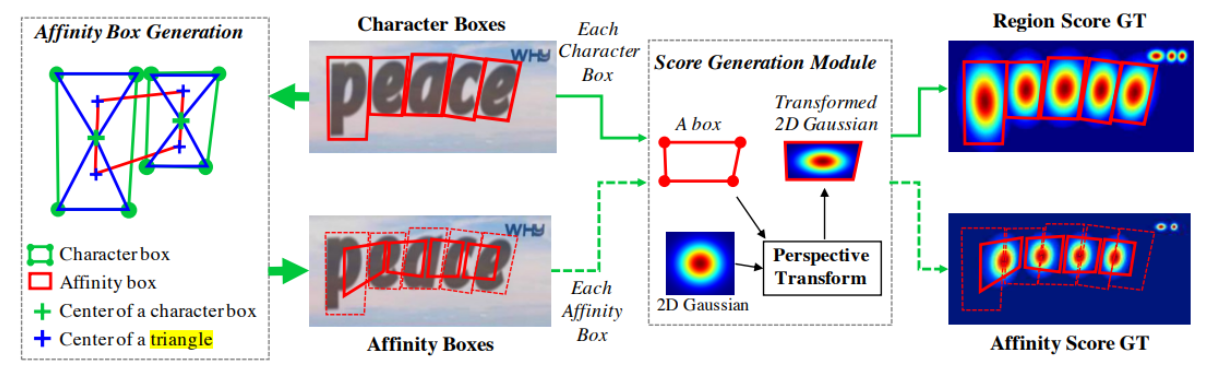
\includegraphics[width=\textwidth]{figs/craft-gt.png}
    \caption{Ilustração das etapas de geração dos arquivos de \textit{ground-truth} para a etapa de treino do CRAFT. Fonte [\citeonline{CRAFT}]}
    \label{fig:craft_gt}
\end{figure}

Para treinar a rede, os autores se utilizaram de uma estratégia de aprendizado levemente supervisionado. Como as principais bases de imagens para treinamento não contam com anotações a nível de caracteres, a rede primariamente é treinada com imagens com texto sintético, usando a base de dados SynthText [\citeonline{SynthText}].

Para refinar o treino em bases de dados com imagens de cenas reais, os autores utilizam a própria rede treinada em texto sintético para predizer as regiões de caracteres das imagens de cena para gerar anotações a nível de caracteres para as imagens das bases de dados utilizados com auxílio de métodos de processamento de imagem, conforme exemplificado na Figura \ref{fig:craft_char_level_annotation}. O processo contém as seguintes etapas:

\begin{itemize}
    \item \textit{Cropping}: Extração das palavras que possuem região descrita nos arquivos de \textit{ground-truth} das bases de dados de avaliação.
    \item \textit{Character Split}: Processo de localização e segregação de cada caractere detectado pela rede treinada em base de dados sintética. A rede a partir das imagens provenientes da etapa de \textit{Cropping}, predizendo as regiões onde a probabilidade de existir um caractere. Com a localização dessas regiões, é aplicado o algoritmo de segmentação conhecido como \textit{Watershed} [\citeonline{WatershedOverview}], cujo objetivo é expandir a área de um caractere a partir do centro da região de maior probabilidade até que as áreas de caracteres adjacentes se encontrem. Isso faz com que seja possível ajustar um \textit{bounding-box} em volta de cada caractere observado.
    \item \textit{Unwarping}: Uma vez em posse da capacidade de localizar todos os caracteres, obtida através da etapa de \textit{Character Split}, pode-se projetar as coordenadas para as \textit{bounding-boxes} de cada caractere de volta para a imagem original aplicando as operações inversas às aplicadas na etapa de \textit{Cropping}
\end{itemize}

Com essas anotações geradas sobre as imagens reais das bases de dados de avaliação, os gabaritos para o treinamento do modelo completo são gerados conforme explicado anteriormente e o treinamento da rede é refinado com esses novos exemplos.

\begin{figure}
    \centering
    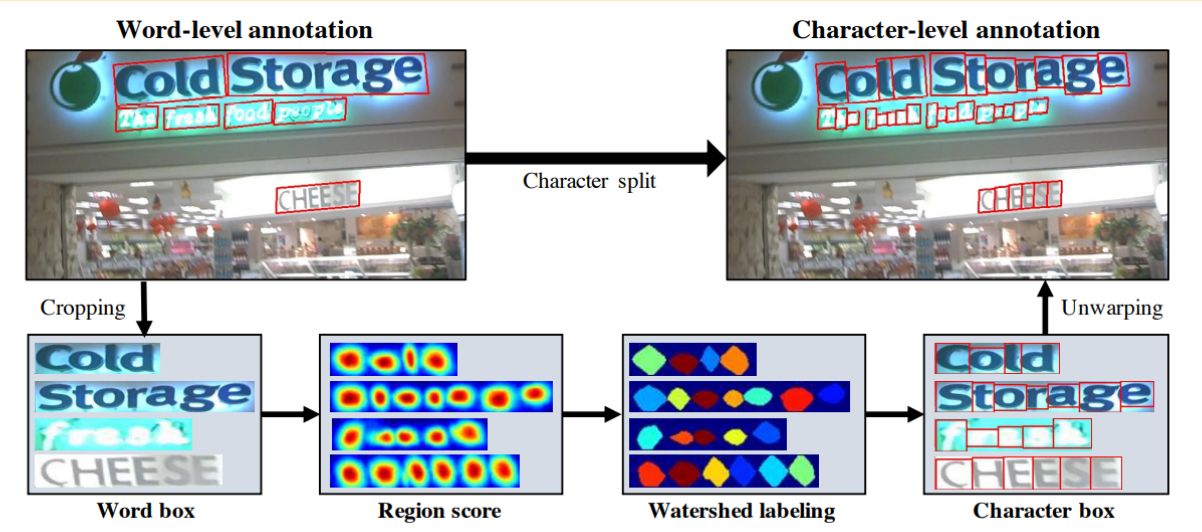
\includegraphics[width=\textwidth]{figs/craft-char-level-annotation.png}
    \caption{Exemplificação do passo a passo para geração de anotações a nível de caracteres durante a etapa de treino do CRAFT. Fonte [\citeonline{CRAFT}].}
    \label{fig:craft_char_level_annotation}
\end{figure}

O CRAFT conta com um pós-processamento bastante simplificado em cima dos mapas de probabilidade que são gerados pela rede com o intuito de calcular os \textit{bounding-boxes} do texto localizado, que envolve, novamente com auxílio de métodos de visão computacional e processamento de imagem. Usando binarização e categorização, é possível unir as regiões de caracteres e de afinidade para extrair as coordenadas dos menores retângulos que encapsulam o resultado dessa união.

%%%%%%%%%%%%%%%%%%%%%%%%%%%%%%%%%%%%%%%%%%%%%%%%%%%%%%%%%%%%%%%%%%%%%%%%%%%%%%%%%%%%%%%%%%%%%%%%%%%%%%%%%%%%%%%%%%%%%%%%

\subsection{Reconhecimento de Texto}
A evolução do segmento de problemas voltados ao reconhecimento de texto, de forma análoga ao avanços observados nas soluções dos problemas de detecção, também acelerou bastante com a popularização do aprendizado profundo. Soluções pré aprendizado profundo faziam extenso uso de pré e pós processamento a partir de extração de características trabalhadas manualmente, como por exemplo HOG [\citeonline{HOG}], aliado classificadores de aprendizado de máquina clássicos. Uma característica da maioria das soluções anteriores a entrada dos métodos de aprendizado profundo é que seguem uma abordagem dita como \textit{bottom-up} [\citeonline{DetcRecogWild}], onde resolvem o reconhecimento a nível de caracteres para então concatenarem os resultados, formando palavras. Outros trabalhos abordaram o mesmo problema pela abordagem inversa, \textit{top-down}, onde a palavra é reconhecida de uma vez só, no entanto apresentam problemas em reconhecer palavras que não fazem parte do dicionario de treinamento da solução.

A partir do uso de redes profundas, algumas linhas para a solução do reconhecimento surgiram, mas a partir do levantamento presente em [\citeonline{DetcRecogWild}] e sugerido por [\citeonline{StrDlEra}], pode-se perceber que grande parte das soluções que já fizeram parte do estado da arte, de alguma forma, se apoiou nas redes convolucionais para codificação e extração de características.
Para atender à característica sequencial do problema de reconhecimento de texto, diversos trabalhos fazem uso de redes neurais recorrentes alimentadas pelos mapas de características resultantes das estruturas convolucionais.

Também por [\citeonline{DetcRecogWild}], observa-se uma dicotomia ao que se refere ao algoritmo de predição empregado pelas soluções do estado da arte. A grande maioria se baseiam em CTC [\citeonline{CTC}], abreviação do nome em inglês \textit{Connectionist Temporal Classification}, e predição baseados em mecanismos de atenção [\citeonline{Attention}].

Para introduzir com um pouco mais de detalhes um dos componentes base do desenvolvimento desse trabalho de graduação, a próxima seção abordará o método CRNN.


%%%%%%%%%%%%%%%%%%%%%%%%%%%%%%%%%%%%%%%%%%%%%%%%%%%%%%%%%%%%%%%%%%%%%%%%%%%%%%%%%%%%%%%%%%%%%%%%%%%%%%%%%%%%%%%%%%%%%%%%

\subsubsection{CRNN} \label{crnn}
\textit{Convolutional Recurrent Neural Networks} [\citeonline{CRNN}], introduzido por \citeauthor{CRNN} é uma solução para o problema de reconhecimento de texto bastante popular, sendo bastante citada em novos trabalhos e sempre presente em trabalhos comparativos. Este método veio para resolver grandes dificuldade das soluções anteriores, por exemplo: lidar com entradas e saídas de comprimentos variados, possibilitar o aprendizado conhecido como fim-a-fim, isto é, aplicar uma função de perda sobre o resultado do reconhecimento e essa perda ser propaganda para o aprendizado da rede extratora de características.

O CRNN, como o nome sugere, une uma rede neural convolucional, sem as camadas de predição totalmente conectadas, para gerar os mapas de características sobre a imagem de entrada. Esses mapas são sequenciados para que alimentem a rede neural recorrente (RNN), que é responsável por conseguir decodificar cada sequência em um possível caractere. A Figura \ref{fig:crnn_pipeline} ilustra o pipeline de processamento que essa arquitetura executa.

\begin{figure}
    \centering
    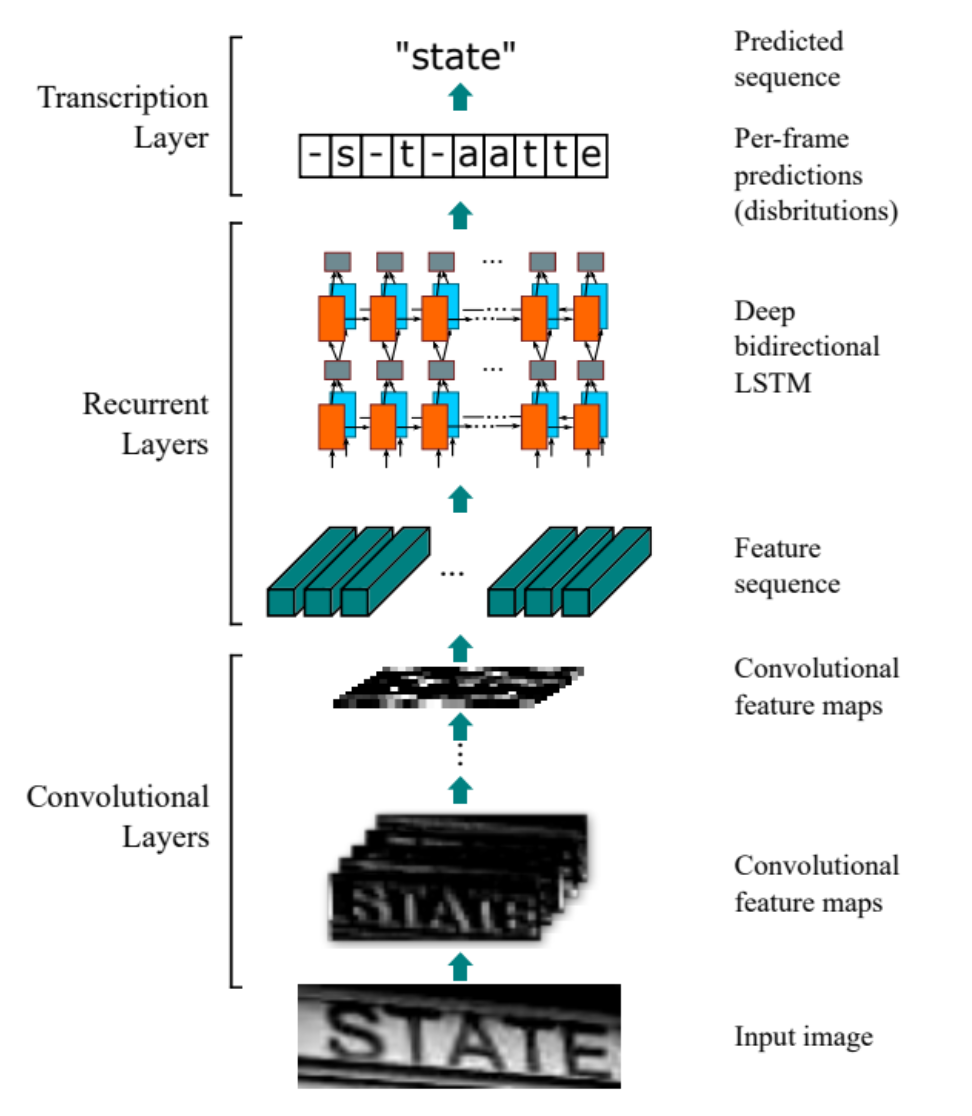
\includegraphics[width=0.75\textwidth]{figs/crnn-pipeline.png}
    \caption{Ilustração do pipeline de reconhecimento do CRNN. Fonte [\citeonline{CRNN}].}
    \label{fig:crnn_pipeline}
\end{figure}

A rede RNN que é implementada no CRNN faz uso de atributos LSTM (\textit{Long-Short Term Memory}) bi-direcional, pois, por visar reconhecer texto em cenas, onde vai existir muita variação na forma de como o texto é observado, muitas vezes carregar o contexto de sequências passadas e futuras é importante para diferenciar caracteres ou possibilitar o reconhecimento de um caractere, por exemplo, uma letra um pouco mais larga.

Os resultados obtidos foram bastante competitivos quando comparados aos métodos de reconhecimento anteriores, até mesmo superiores aos que já faziam uso dos conceitos de aprendizado profundo, com o adicional de prover meios de aprendizado integrado da rede convolucional e recorrente como uma unidade, além de um modelo bem mais enxuto em número de parâmetros [\citeonline{CRNN}].

Por lidar com o reconhecimento como um problema de sequência, o modelo pressupõe que a orientação do texto é necessariamente da esquerda para a direita, isso leva a uma limitação, que seria reconhecer textos com não exatamente horizontais e retilíneos.

%%%%%%%%%%%%%%%%%%%%%%%%%%%%%%%%%%%%%%%%%%%%%%%%%%%%%%%%%%%%%%%%%%%%%%%%%%%%%%%%%%%%%%%%%%%%%%%%%%%%%%%%%%%%%%%%%%%%%%%%